%!TEX root = Main.tex
\section{Purpose}

To ensure that the scenario can be implemented to an existing system, it is important not to rewrite code of the existing system, but add to it, thus not breaking it for other developers.
The Common Ambient Assisted Living Homecare Platform, CAALHP, is a framework which behaves as a Context-Awareness system, just like the Java Context-Awareness Framework\cite{JCAF}, JCAF.
JCAF is built upon layers to ensure functionality and responsibility is divided to those who should handle it, allowing devices monitoring service by subscribing to them, letting services subscribe to devices and publish data to the monitors.
Another context framework implementing this technique is the Context Toolkit\cite{ContextToolkit}, which consist of several types of class, including \texttt{interpreters} to convert context to higher level information, and \texttt{discoverers} to register capabilities in the framework.

By using an object oriented model, a service for CAALHP (written in C\#) will be able to use inheritance, objects, an encapsulations to represent the data retrieved from the sensor and present them to monitors or other services, much as show on Figure \ref{fig:JCAF}.
The service will be automatically added to the CAALHP with context discoverers.

\begin{figure}[hbtp]
	\centering
	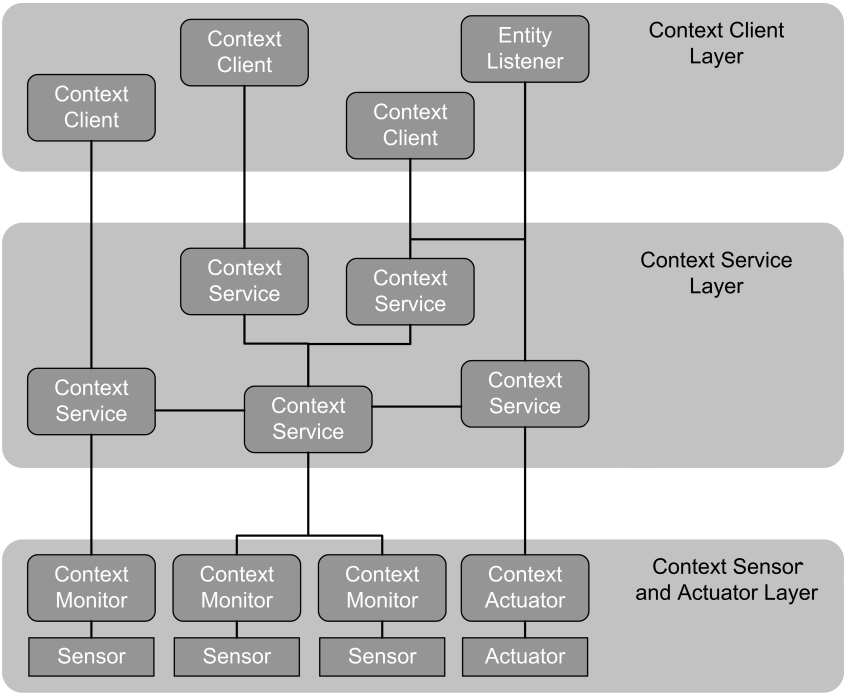
\includegraphics[width = 0.48 \textwidth]{JCAF}
	\caption{JCAF hierarchi\cite[5]{JCAF}. 
	Sensors are monitored by context monitors, which will provide the Context Service Layer with data from the sensors.
	The Context Services can subscribe to any number of Context Monitors and other Context Services, to calculate and present data for Context Clients, which can trigger alarms, display data for a user etc.}
	\label{fig:JCAF}
\end{figure}

The CAALHP is an Open Source project\cite{BB-CAALHP} which already operates with several different sensors and services.
Adding functionality must not affect other parts of the system -- it must run by it self, subscribing to the types of events coming into the system, and providing and API for the data the service handles.

With Open Source projects the important part is, that other developers can use it as well, e.g. integrate it into their own system or adopt the project to work on.
Implementing new functionality to an existing solution should not break the solution, only enhance it. 
If new sensors and detectors are to be implemented to the system it should comply with these rules (if possible) and allow for other developers to use them as well.
Selecting hardware to use with the system is therfore an important task, because hardware can be bound to software which are not compatible / unaccessable.

I called different companies and asked for their solutions, and whether their hardware would be implementable with the CAALHP.
Table \ref{tab:Compare} shows different product from different companies, how they match up pricewise and whether they are compatible with the CAALHP based on phone conversations with employees at each company.

\begin{table}[htbp]
\centering
\begin{tabular}{cccc}
\textbf{Company}  & \textbf{Product} & \textbf{Compatible} & \textbf{Priciness} \\ \hline
\rowcolor{gr} 
Tunstall  & Intelligent ceiling\cite{Tun-Loft} & Yes & Semi expensive \\
Tunstall  & Bed Guard\cite{Tun-bed} & Yes & Cheap \\
\rowcolor{gr} 
MariCare & Intelligent floor\cite{Elsi}  & Maybe & Very expensive \\ 
Yes Group & Bed Guard\cite{YG-bed} & Yes & Cheap \\
\rowcolor{gr} 
AnyGroup & Bed Guard\cite{AnyGroup-bedguard} & API not open yet. & Cheap\\
AnyGroup & Multi Guard\cite{AnyGroup-multiguard} & API not open yet. & Cheap \\\hline
\end{tabular}
\caption{Different companies products, price range and compatibility.}
\label{tab:Compare}
\end{table}

The company Tunstall provides many sensors of various art.
The two products in Table \ref{tab:Compare} is related to this project as they too can tell if a person is in bed and if a person might have fallen.
All Tunstall's products communicates through a protocol they call \textit{CT-Link}, which have an open API.
Their products' prices varies but the more units run through the CT-Link, the easier it might be to implement it to the CAALHP.

MariCare provides an intelligent floor solution, which acts as a huge tablet screen regarding to pressure points, and is able to detect if you have fallen.
The hardware is required to be placed under the floor and is therefore very expensive to install in buildings.
They could not tell if the API was open.

Yes Group produces bed guards, small PIR sensors to detect if you have moved from the bed or not.
They have a open API and are cheap to buy.

AnyGroup, a sister company to Yes Group, produces a wider range of sensor, among them bed guards.
They have an API but it is not open yet. 
The units are cheap however.